\chapter{Web of Things}
\label{web-of-things}

\section{Web of Things vs Internet of Things}

\textbf{Internet of Things definition} \\

The Internet of Things (IoT) is a system of physical objects that can be
discovered, monitored, controlled or interacted with by electronic devices
which communicate over various networking interfaces, and eventually can be
connected to the wider Internet. \\

There's a new class of objects that is about to come into our houses:
\textbf{Smart Things}. A Smart Thing is a physical object that is digitally
augmented with one or more of the following:

\begin{itemize}
  \item Sensors (temperature, light, motion, etc.)
  \item Actuators (displays, sound, motors, etc.)
  \item Computation (can run programs and logic)
  \item Communication interfaces (wired or wireless)
\end{itemize}

\begin{figure}[H]
  \centering
  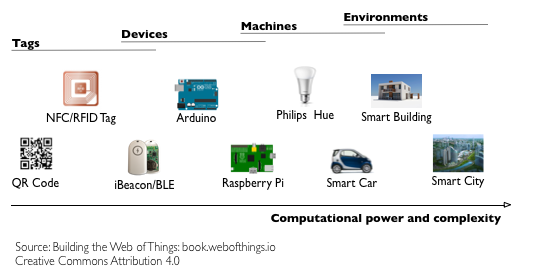
\includegraphics[scale=0.6]{iotland.png}
  \caption{The IoT landscape. The IoT is a network of Things, which are
anything that can be connected in some form to the Internet.}
  \label{fig:iotland}
\end{figure}

The Internet part simply means that the Thing (its services or data about/from
it) can be accessed and processed by other applications through the existing
Internet infrastructure.

The limitations of the IoT become obvious as soon as one wants to integrate
devices from various manufacturers into a single application or system.

\begin{figure}[H]
  \centering
  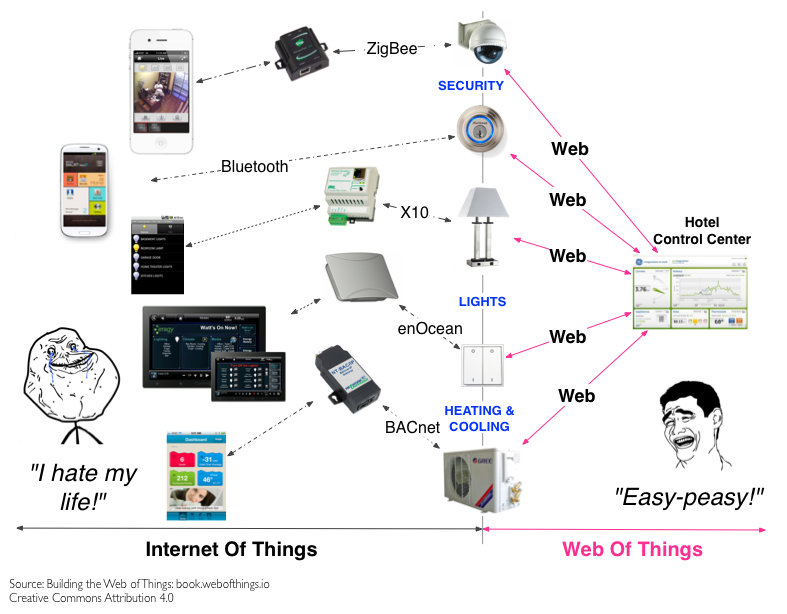
\includegraphics[scale=0.5]{integration_problem.png}
  \caption{In the IoT, hundreds of incompatible protocols co-exist today.
This makes the integration of data and services from various devices extremely
complex and costly.}
  \label{fig:integration_problem}
\end{figure}

\subsection{Breaking the ``one device, one protocol, one app'' pattern}

In the Web of Things (not IoT!), any device can be accessed using standard Web
protocols.

Connecting heterogeneous devices to the Web makes the integration across
systems and applications much simpler.

The idea of maximizing existing and emerging tools and techniques used on the
Web and apply them to the development of IoT scenarios is what we call the Web
of Things.

While the IoT has been busy resolving networking problems, the Web of Things
relies exclusively on application level protocols and tools.

Mapping any device into a Web mindset makes the Web of Things agnostic to the
physical and transport layer protocols used by devices.

\begin{figure}[H]
  \centering
  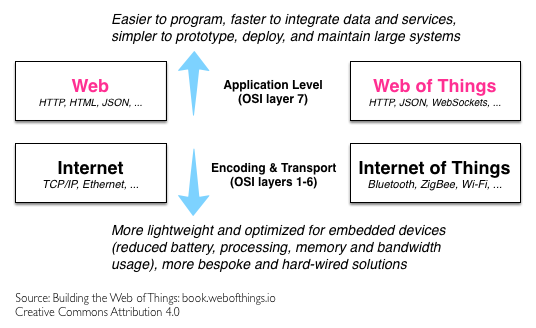
\includegraphics[scale=0.6]{iotstack.png}
  \caption{The Web of Things only deals with the highest OSI Layer, which
handles applications, services and data.
Working on such a high level of abstraction makes it possible to connect data
and services from many devices regardless of the actual transport protocols
used.
In contrast, the Internet of Things does not advocate (sostiene) a particular
application level protocol and is usually focusing on the lower layers of the
OSI stack.}
  \label{fig:iotstack}
\end{figure}

\textbf{The goal is access the Things in a standard and transparent
way.}

\begin{figure}[H]
  \centering
  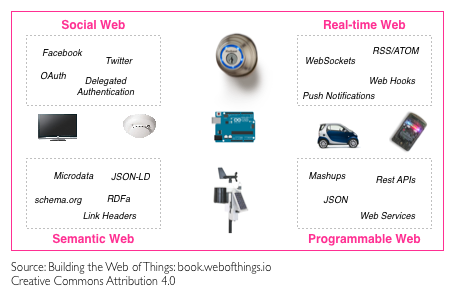
\includegraphics[scale=0.7]{iotweb.png}
  \caption{The Web of Things is the ability to use modern Web standards
directly on embedded devices.}
  \label{fig:iotweb}
\end{figure}

This makes the Web the ideal substrate for building a ``universal''
architecture and Application Programming Interface (API) to interact with
Things.

In practice, this means that the user can start interacting with Things via Web
browsers and explore the Web of Things just as he would surf the Web (via links
to other related things).
Real-time data collected from distributed sensors can then be easily retrieved,
processed, and displayed on Web pages using HTML, CSS and JavaScript.

\begin{figure}[H]
  \centering
  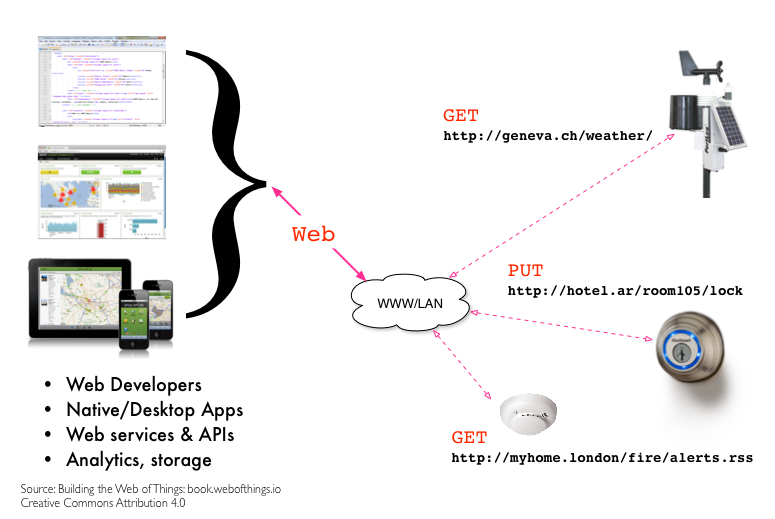
\includegraphics[scale=0.5]{iotrest.png}
  \caption{A URL for each thing and a RESTful API.
The Web of Things allows developers and applications to exchange data with any
device using standard HTTP/WebSockets requests, regardless of how the device is
connected.}
  \label{fig:iotrest}
\end{figure}

\textbf{BUT} although Web protocols are available and usable for IoT devices,
they may be too heavy for some IoT applications. Let's have a look to others
protocols.

\subsection{Not all speak HTTP}

\textbf{MQTT}\\

MQ Telemetry Transport (MQTT) is an open source protocol for constrained
devices and low-bandwidth, high-latency networks.
It has a publish/subscribe messaging transport that is extremely lightweight
and ideal for connecting small devices to constrained networks.
MQTT is bandwidth efficient, data agnostic, and has continuous session
awareness. It helps minimize the resource requirements for an IoT device,
while also attempting to ensure reliability and some degree of assurance of
delivery with grades of service.\\

\textbf{Properties:}

\begin{itemize}
  \item client/server model, where every sensor is a client and connects to a
server (a.k.a. broker)
  \item clients subscribe to topic channels of interest
  \item topic channels are hierarchical (e.g., room2BC/heating)
  \item 3 QoS Levels: ``Fire and forget'',  ``delivered at least once'' and
 ``delivered exactly once''.
  \item username/password authentication
  \item TCP over SSL/TLS
\end{itemize}

\textbf{CoAP}\\

The Constrained Application Protocol (CoAP) was designed for use with low-power
and constrained networks. CoAP is a RESTful protocol. It is semantically
aligned with HTTP, and even has a one-to-one mapping to and from HTTP.\\

\textbf{Properties:}

\begin{itemize}
  \item packets are much smaller than HTTP TCP flows
  \item simpler and faster to parse with small memory footprint
  \item over UDP, interoperates with HTTP and the RESTful web through simple
proxies
  \item client/server model where clients may GET, PUT, POST and DELETE
resources
  \item DTLS capable CoAP devices support RSA and AES or ECC and AES
\end{itemize}

\begin{figure}[H]
  \centering
  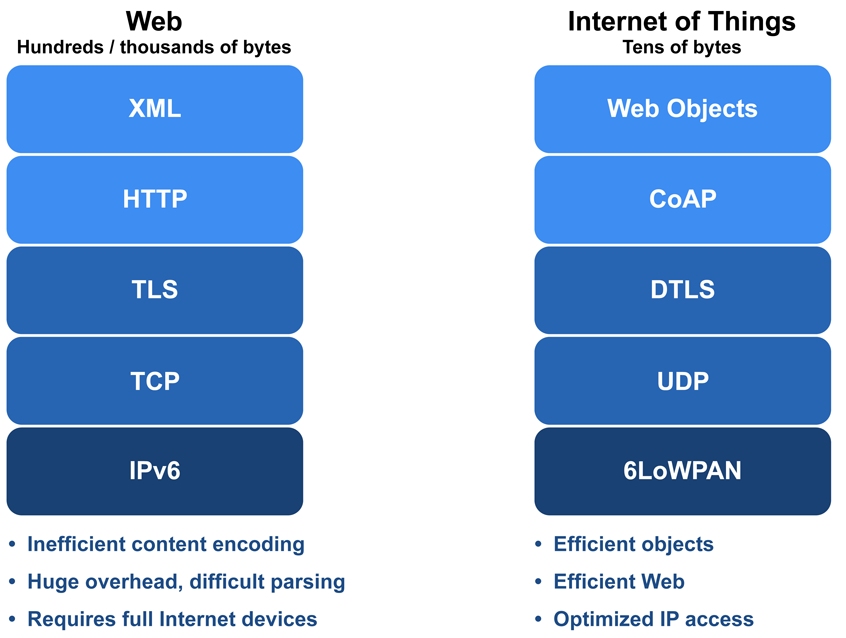
\includegraphics[scale=0.4]{protocol_comparison.png}
  \caption{On the left, the protocol stack for Web applications can easily
produce a data overhead of hundreds or thousands of bytes.
By comparison, IoT protocols are optimized for constrained devices and
networks, and produce a much smaller data overhead of tens of bytes.}
  \label{fig:protocol_comparison}
\end{figure}

\subsection{Integration Patterns}

\textbf{Direct Communication}

In the most straightforward case, a Web Thing is simply a Web API that Clients
send requests to.
The Client and the Web Thing can be on the same network or on different
networks.

\begin{figure}[H]
  \centering
  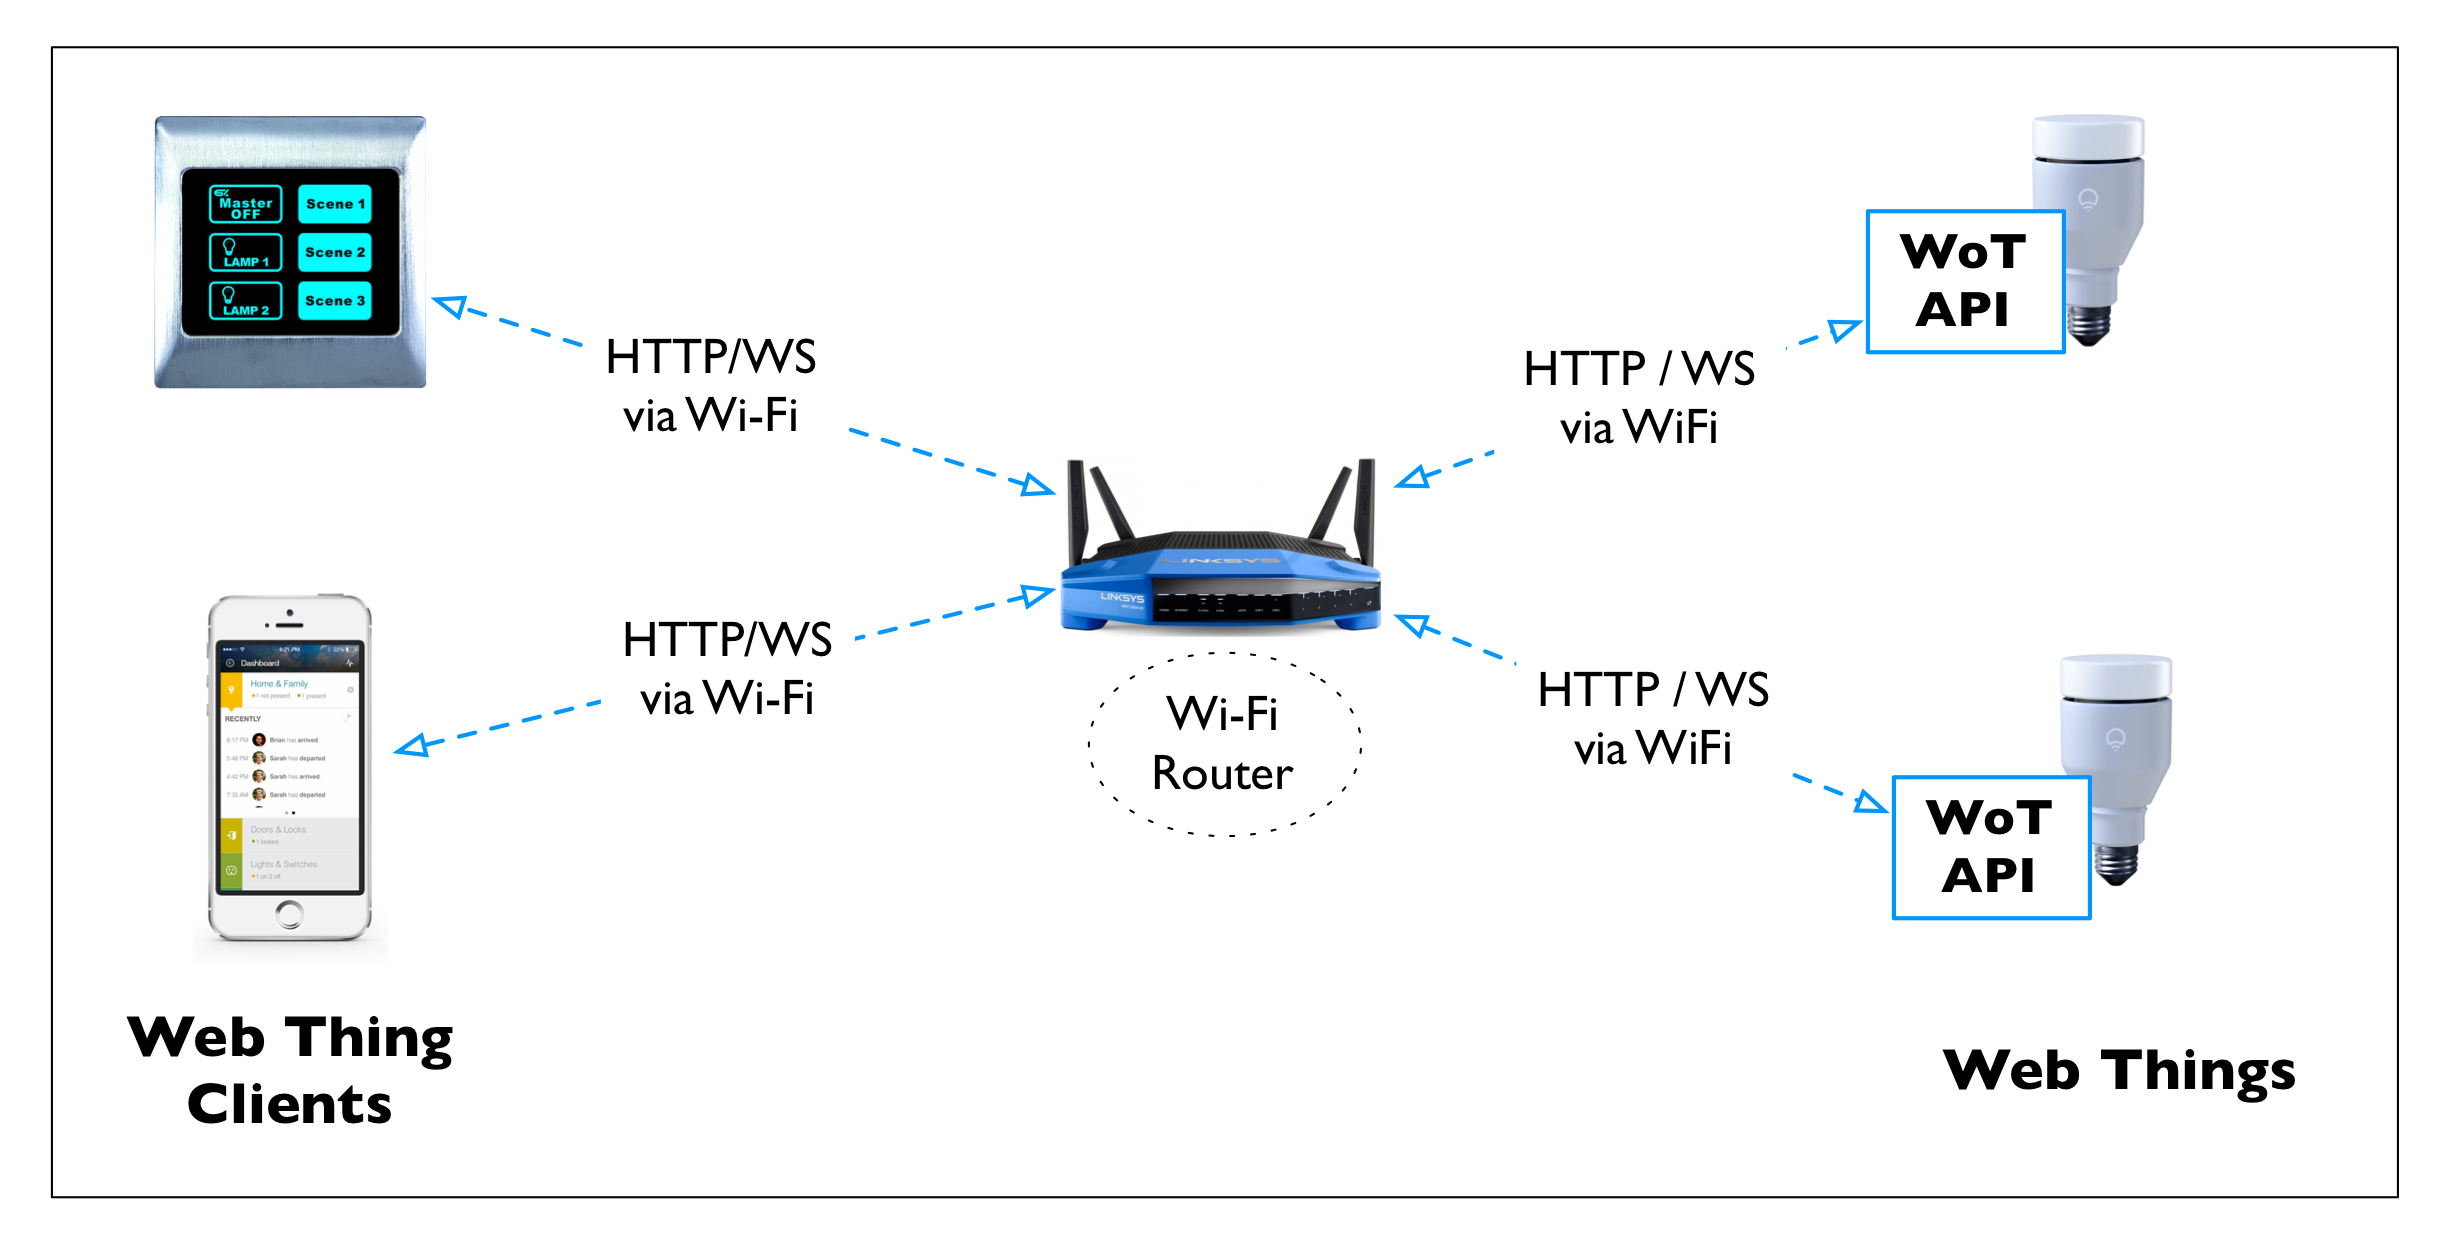
\includegraphics[scale=0.5]{direct_communication.png}
  \caption{Direct connectivity between a Client and a Web Thing}
  \label{fig:direct_communication}
\end{figure}

\textbf{Gateway}

Gateway-based connectivity is used when a Thing cannot offer a Web API
directly.

In this case an intermediate Web Thing - the gateway - exposes a Web API on the
Thing's behalf (per conto di).
The Web Thing therefore acts as a proxy for the Thing (or gateway depending on
the complexity/layer of the translation).

\begin{figure}[H]
  \centering
  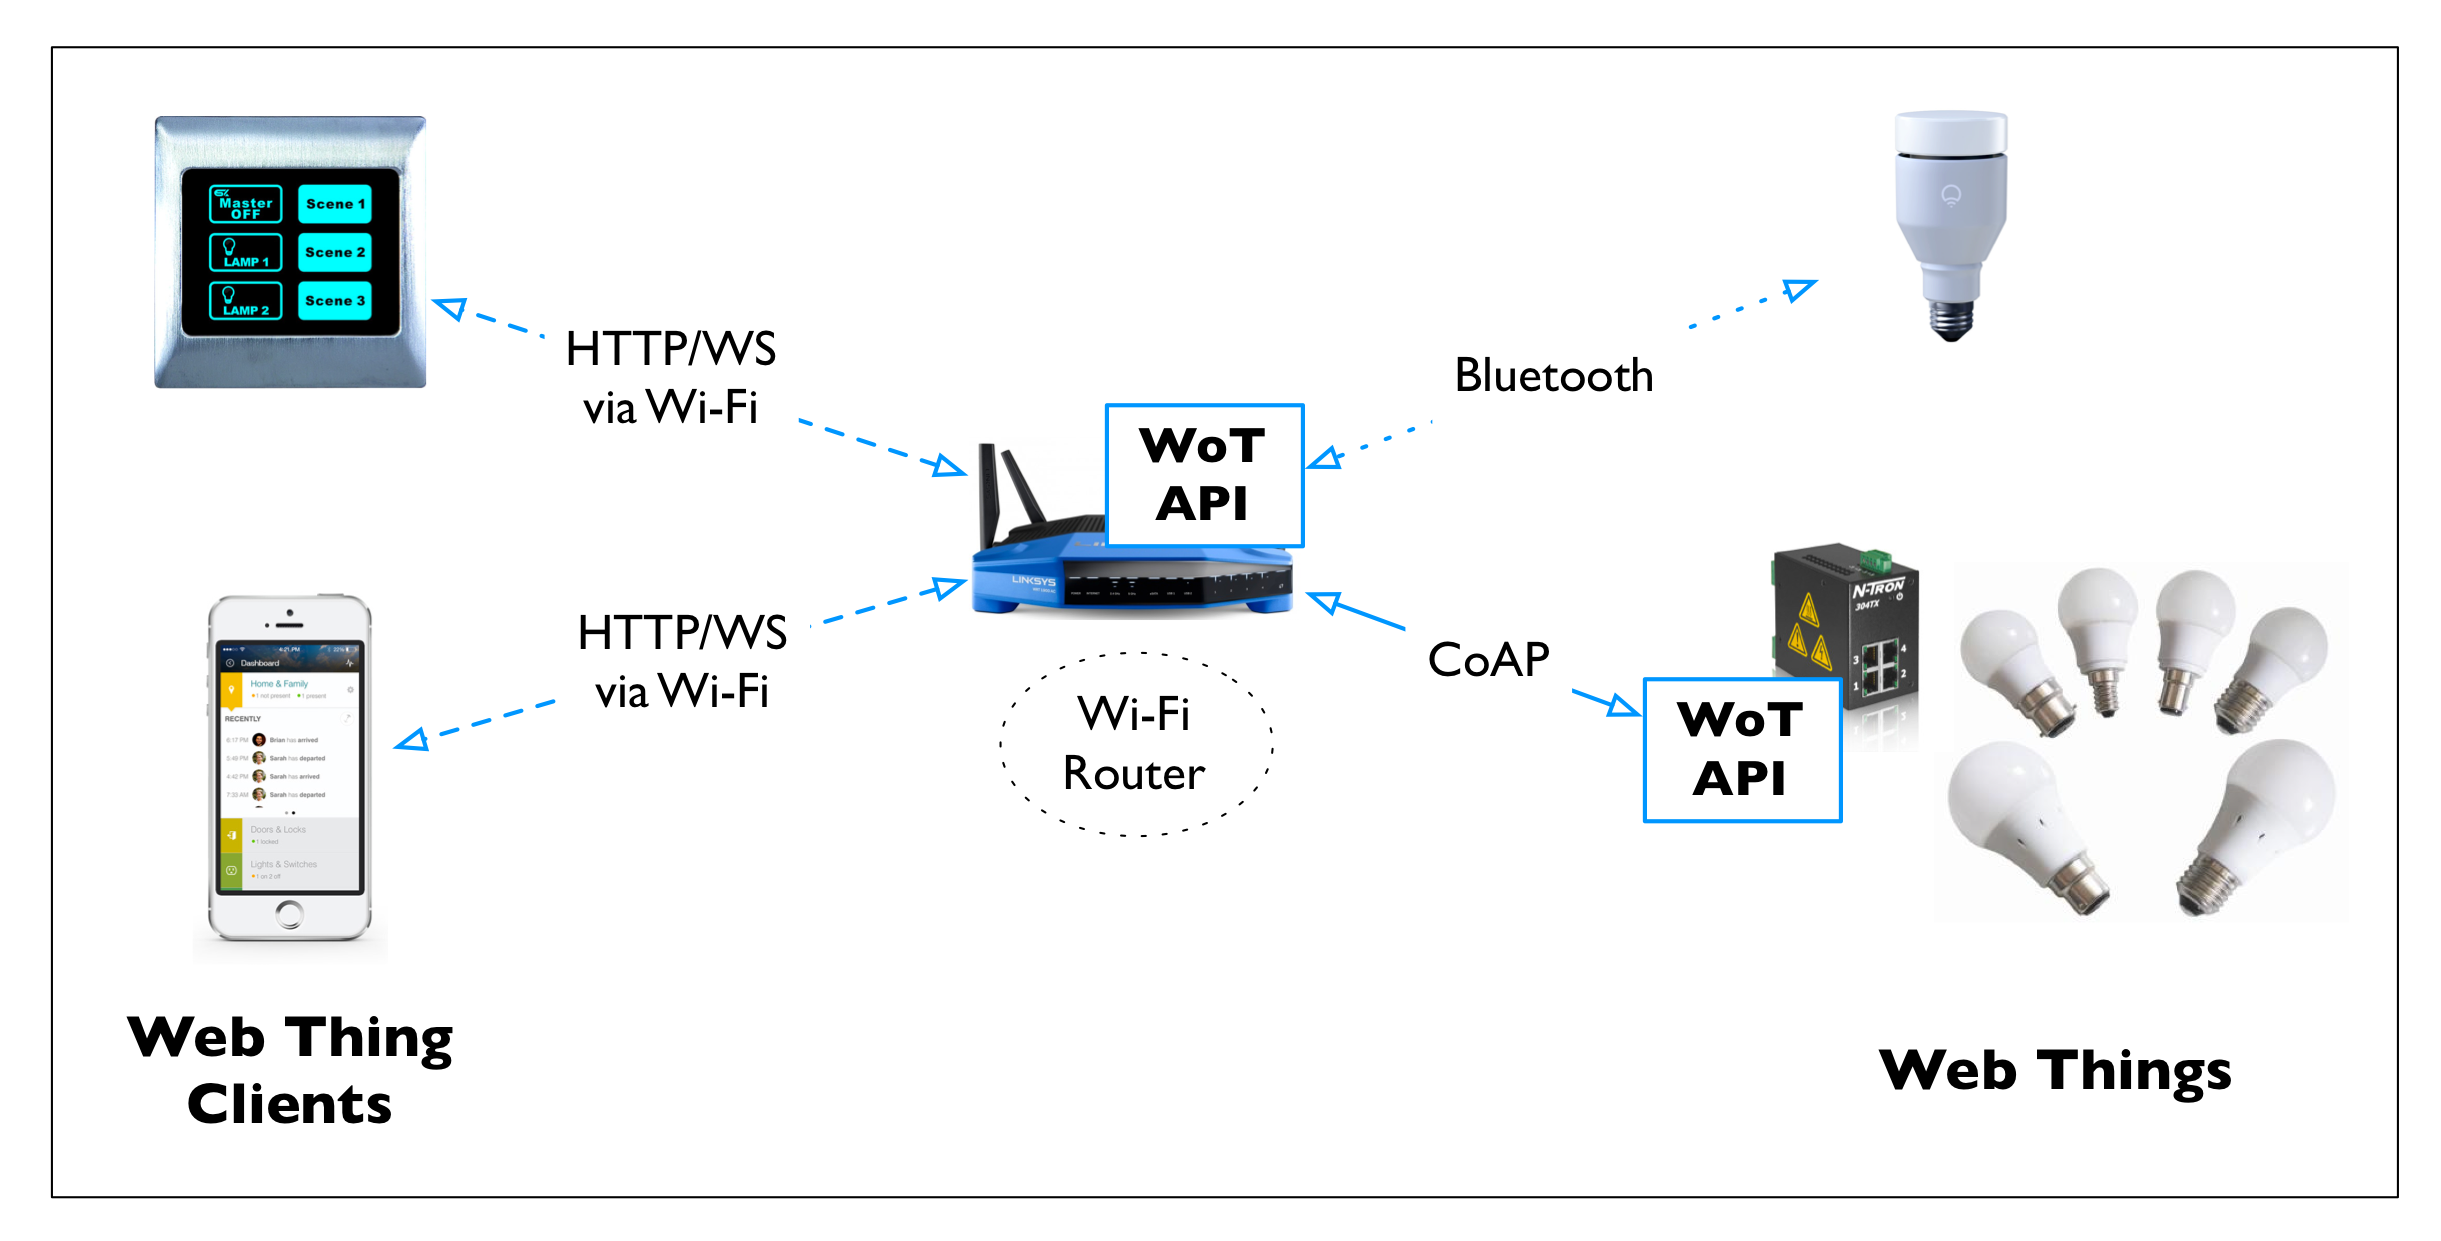
\includegraphics[scale=0.5]{gateway.png}
  \caption{Gateway-based connectivity between a Client and a Web Thing}
  \label{fig:gateway}
\end{figure}

\textbf{Cloud}

This third case is similar to the previous case. However, this time the gateway
is a cloud service.

\begin{figure}[H]
  \centering
  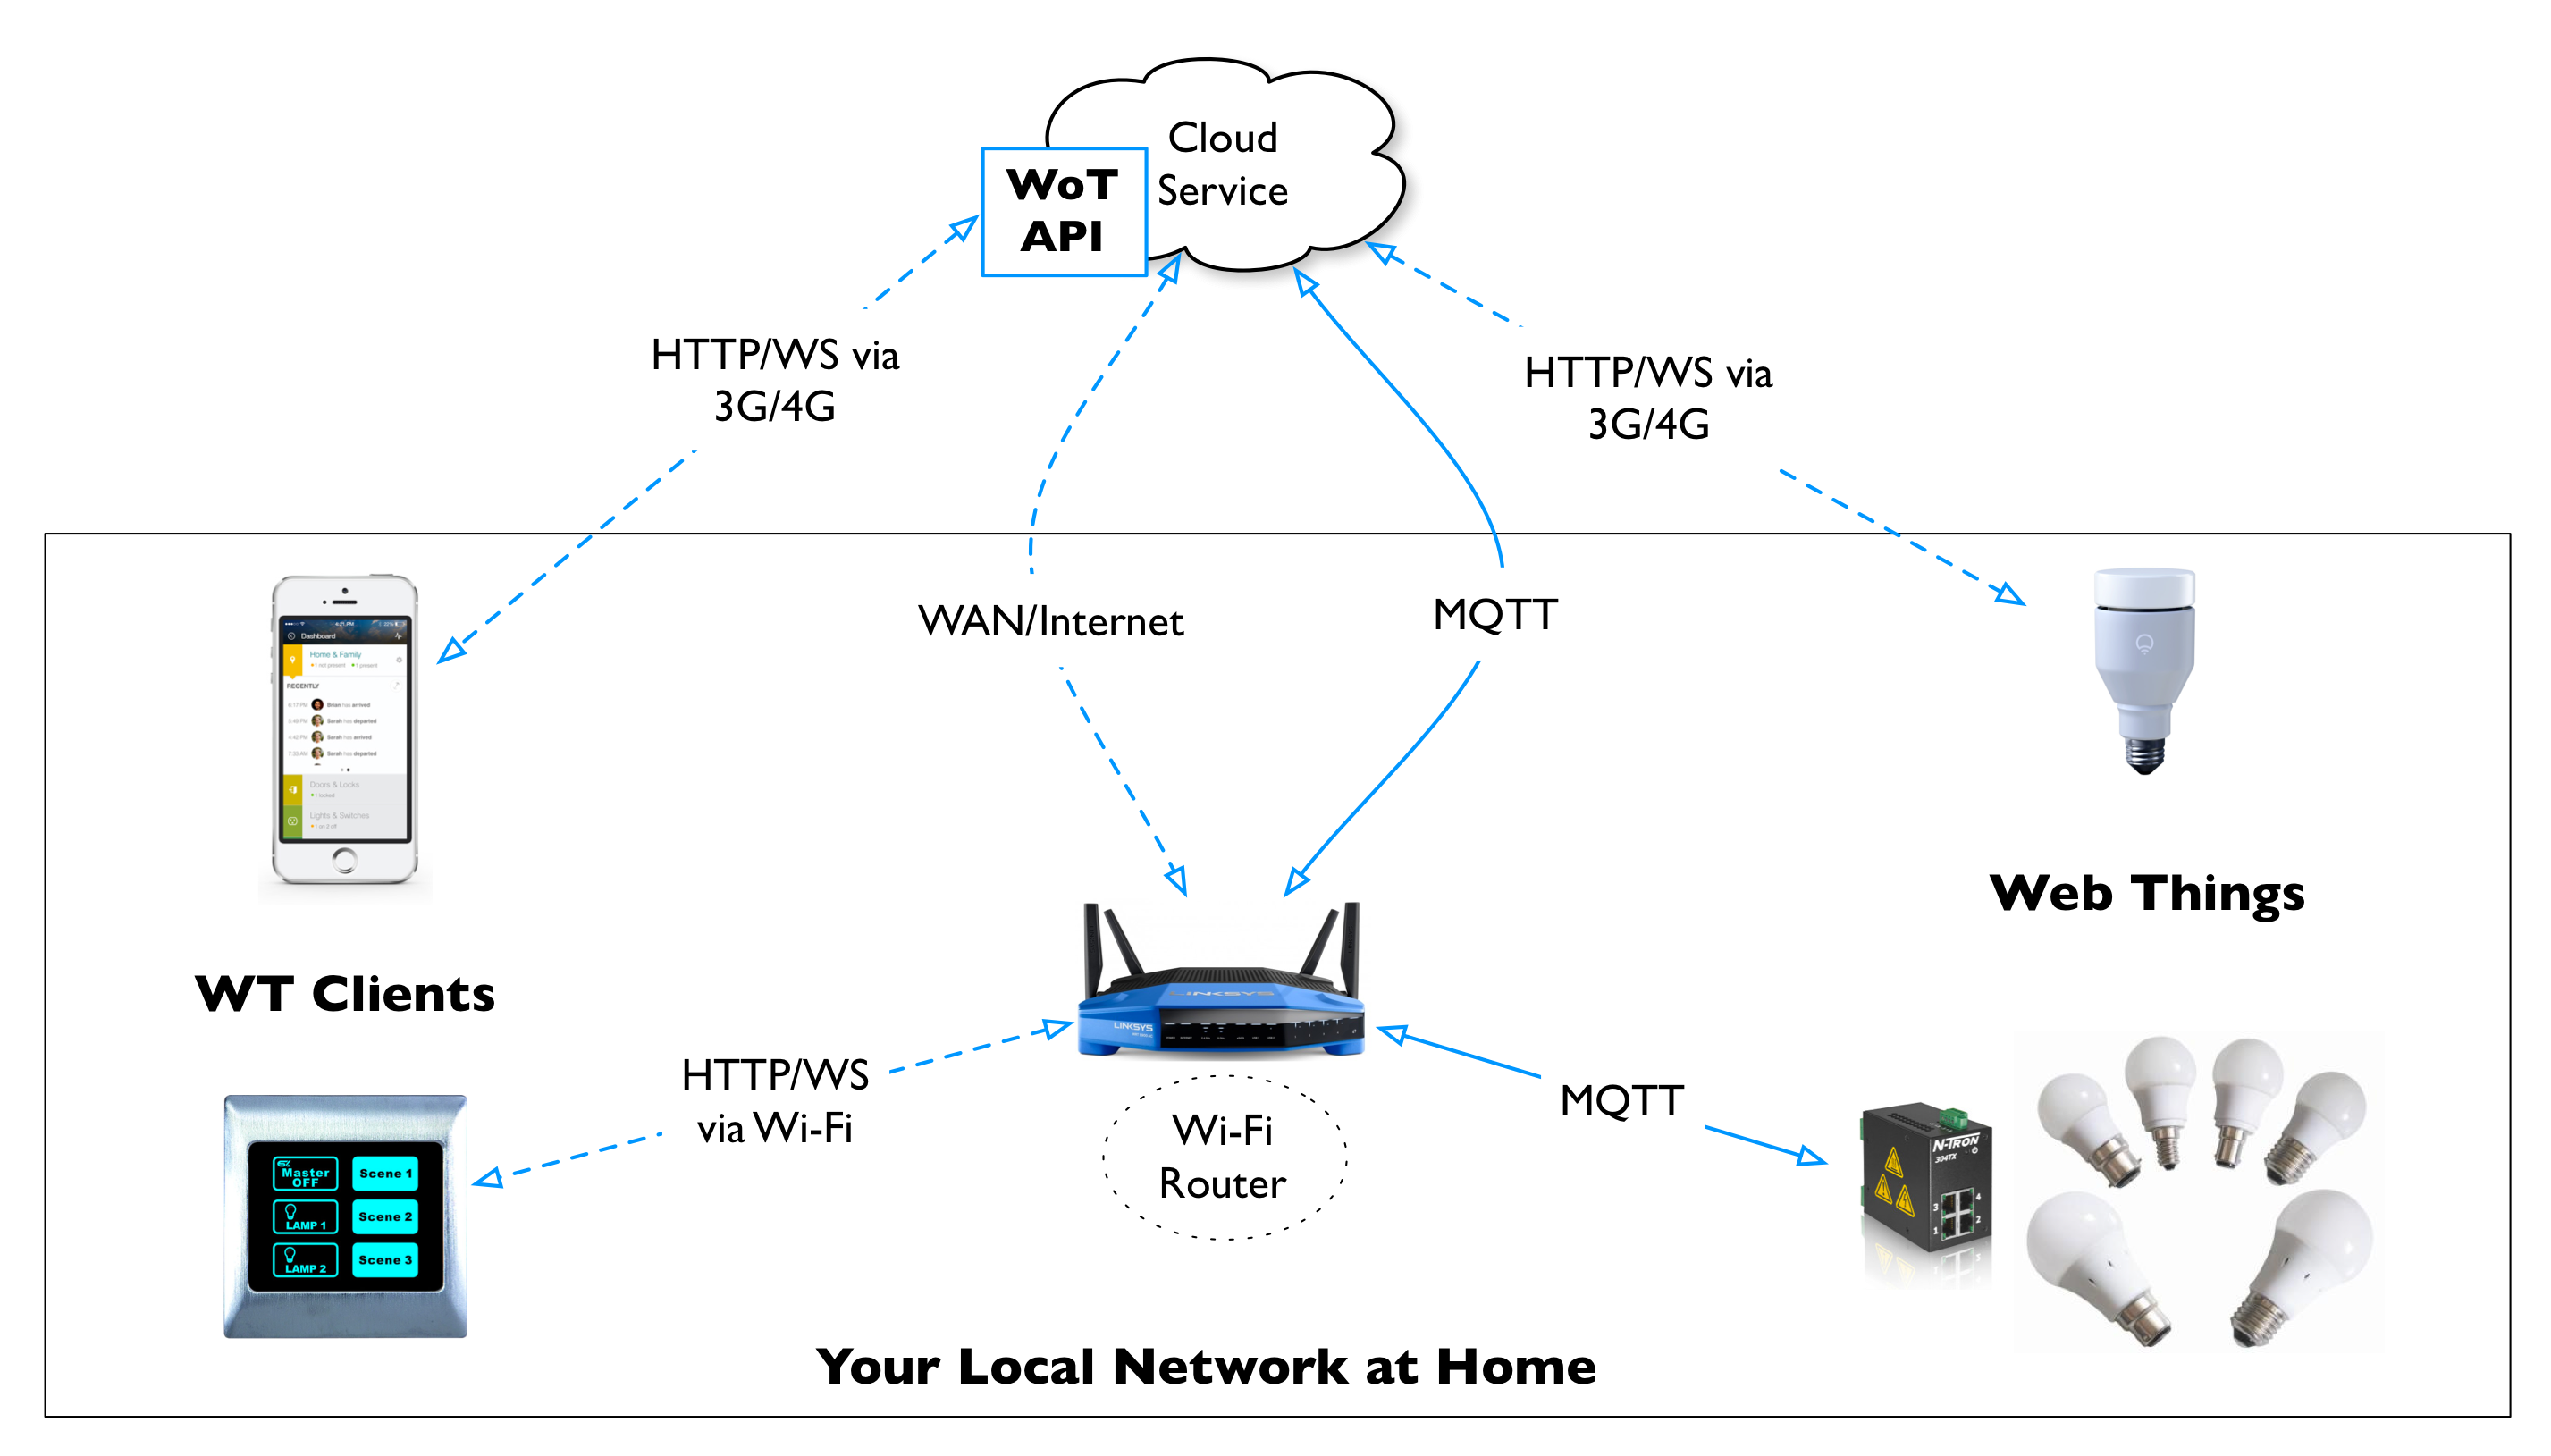
\includegraphics[scale=0.5]{cloud.png}
  \caption{Cloud-based connectivity between a Client and a Web Thing}
  \label{fig:cloud}
\end{figure}

\subsection{Web of Things Architecture}

While there are ongoing efforts to standardise it, the Web of Things is a set 
of best practices that can be classified according to the Web of Things
architecture.
The architecture proposes four main layers that are used as a framework to
classify the different patterns and protocols involved.

\begin{figure}[H]
  \centering
  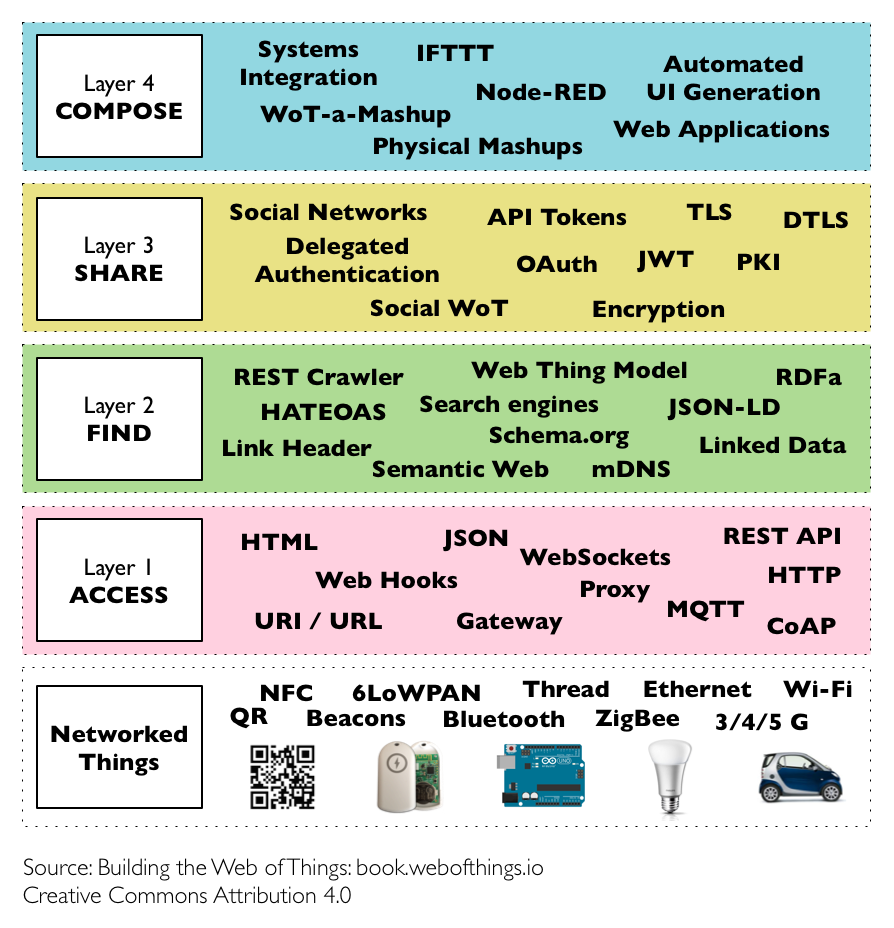
\includegraphics[scale=0.5]{wotarchitecture.png}
  \caption{Web of Things Architecture}
  \label{fig:wotarchitecture}
\end{figure}

\textbf{Accessibility layer}\\

This layer deals with the access of things to the
Internet and ensure they expose their services via Web APIs
(already discussed in the previous sections of this chapter).\\

\textbf{Findability layer}\\

Marking things accessible via an HTTP and WebSocket API is great but it doesn't
mean applications can really  ``understand'' what the Thing is, what data or
services it offers, and so on.

This is where the second layer – Find – becomes interesting.
This layer ensures that your Thing can not only be easily used by other HTTP
clients but can also be findable and automatically usable by other WoT
applications.

The approach here is to reuse web semantic standards to describe things and
their services.

This enables searching for things through search engines and other web indexes
as well as the automatic generation of user interfaces or tools to interact
with Things.\\

\textbf{Sharing layer}\\

The Internet of Things will only blossom (fiorirà) if Things have a way to
securely share data across services.

This is the responsibility of the Share layer, which specifies how the data
generated by Things can be shared in an efficient and secure manner over
the web.

At this level, another batch of Web protocols help.
First, TLS, the protocol that makes transactions on the Web secure.
Then, techniques such as delegated web authentication mechanisms like OAuth
which can be integrated to our Things' APIs. Finally, we can also use social
networks to share Things and their resources to create a Social Web of
Things.\\

\textbf{Composition layer}\\

Finally, once Things are on the Web (layer 1) where they can be found by humans
and machines (layer 2) and their resources can be shared securely with others
(layer 3), it's time to look at how to build large-scale, meaningful
applications for the Web of Things. In other words, we need to understand the
integration of data and services from heterogeneous Things into an immense
ecosystem of web tools such as analytics software and mashup platforms.
Web tools at the Compose layer range from web toolkits - for example,
JavaScript SDKs offering higher-level abstractions - to dashboards with
programmable widgets, and finally to physical mashup tools such as Node-RED as
shown below.

\begin{figure}[H]
  \centering
  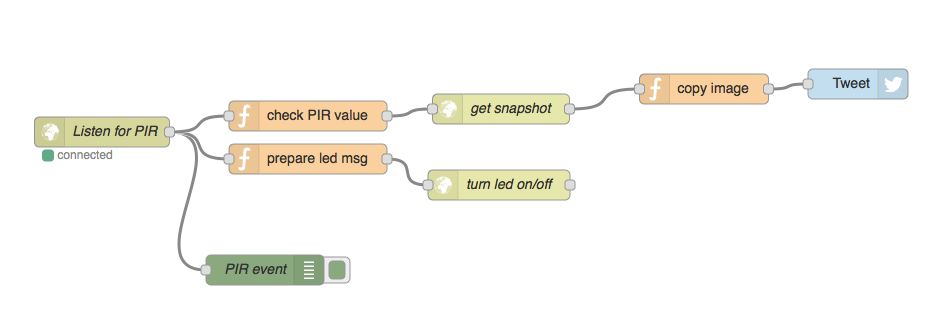
\includegraphics[scale=0.4]{nodered.png}
  \caption{A Physical Mashup with Node-RED;
Monitor a process / sensor;
Automatic control of heating system;}
  \label{fig:nodered}
\end{figure}

\subsubsection{Conclusion}

The Web of Things is a high-level application protocol designed to maximize
interoperability in the IoT. Web technologies are widely popular and offer all
the flexibility and features needed for the majority of future IoT
applications, including discovery, security, and real-time messaging.\\

\textbf{Sources:}\\

A mix of:

\begin{itemize}
  \item Course slides
  \item \url{http://webofthings.org/2016/01/23/wot-vs-iot-12/}
  \item \url{http://webofthings.org/2017/04/08/what-is-the-web-of-things/}
  \item \url{https://www.micrium.com/iot/internet-protocols/}
  \item \url{https://www.w3.org/blog/wotig/}
\end{itemize}
